The following four models were constructed: 
\begin{enumerate}
    \item Long Short-Term Memory (LSTM)
    \item Multi-Layer Perceptron (MLP)
    \item LightGBM (LGBM)
    \item LSTM-LGBM Hybrid
\end{enumerate}
Bayesian optimization was used to optimize the hyperparameters of the models within a given range of values.
The optimization process consisted of a few rounds of exploration, where new points are randomly explored within the available space, and many rounds of exploitation, where Bayesian optimization is done to find the optimal hyperparameters.
The performances of the optimized models were evaluated on the training, validation and test sets for a 1-day ahead point forecast and were compared to the performance of a naive model.
Moreover, the performance of each optimized model was evaluated on the test set for a 28-days ahead point forecast and compared to the naive model.
The ME, RMSE, and RMSSE of each model after hyperparameter optimization on the training, validation, and test sets are shown in tables \ref{tab:lstm_results}, \ref{tab:ann_results}, \ref{tab:lgbm_results}, \ref{tab:hyb_results}.
Note that for the MLP and LGBM models, the 1-day ahead forecasts are the same as the 28-days ahead forecasts, but for the LSTM and hybrid models, these forecasts are different.
This is due to the difference in the feature engineering done for the LSTM and hybrid models compared to the MLP and LGBM models, which will be discussed further in the discussion.
% talk more about which model fitted best on the trn/val/tst sets. whether it was able to generalize as well?
From the results, it can be seen that the LGBM model outperforms the other models with an RMSSE of \lgbmTstMonRMSSE{} on the test set for 28-days ahead forecasts.

In the rest of this chapter, the results of hyperparameter optimization and the performance of each model on the training, validation, and test sets will be discussed in detail. 

\section{Long Short-Term Memory}
\InsertBoxR{3}{
    \parbox{0.5\linewidth}{
    \vspace{4mm}
    \captionsetup{width=0.49\textwidth}
    \fbox{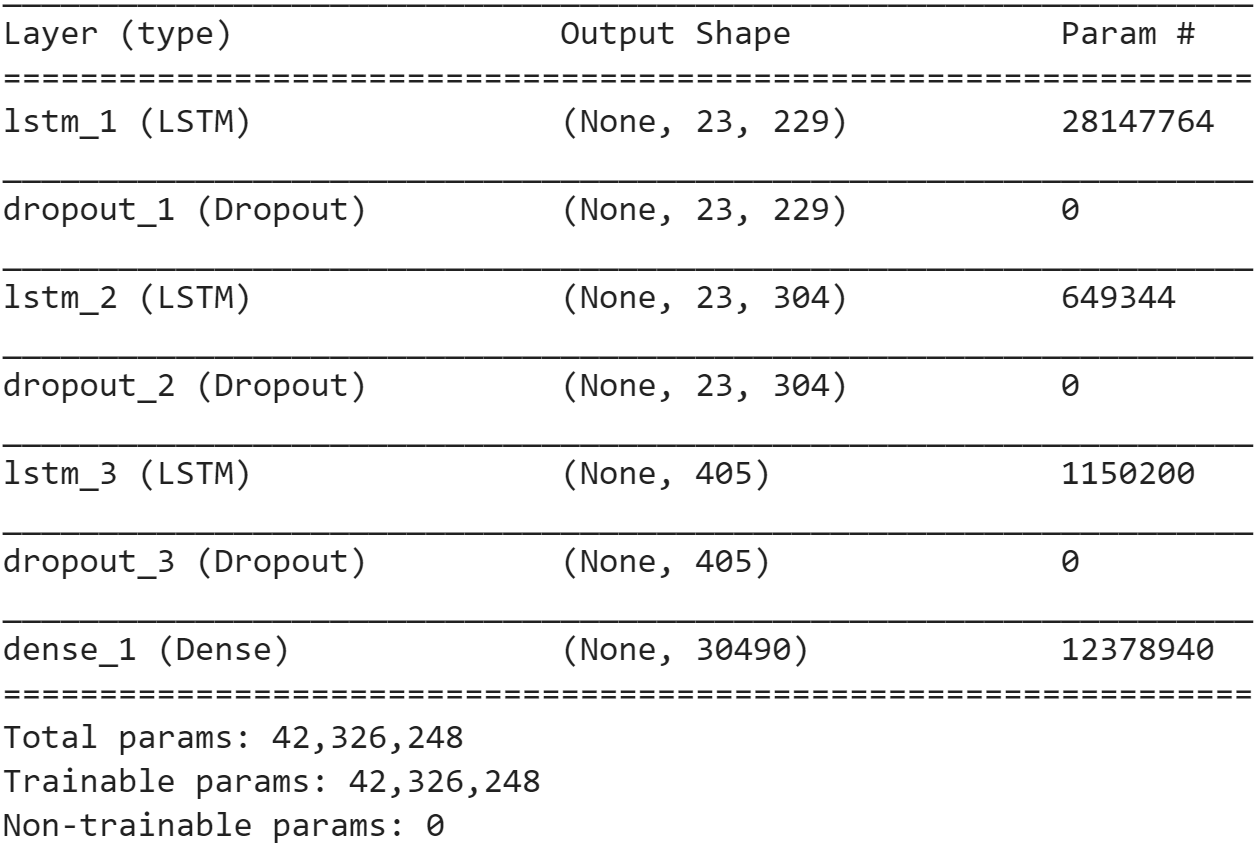
\includegraphics[width=0.47\textwidth]{figures/results/lstm_summary.PNG}}
    \captionof{figure}{A summary of the LSTM's structure.}
    \label{fig:lstm_summary}}}[3]
Figure \ref{fig:lstm_summary} shows a summary the LSTM model's structure. 
The LSTM model was able to achieve an RMSE of \lstmTrnRMSE{} on the training set, \lstmValRMSE{} on the validation set, and \lstmTstRMSE{} on the test set, when predicting one day ahead. 
Moreover, the RMSE of the model on the test set for 28-days ahead forecasts was \lstmTstMonRMSE{}.
Figure \ref{subfig:lstm_sample1} shows the 1-day ahead predictions of the LSTM model versus the actual sale values for the last 28 days of the training set, as well as the entire validation and test sets, which shows that the model was able to learn the weekly pattern presented in the time-series data.
The 28-days ahead predictions of the model on the test set are also shown in Figure \ref{subfig:lstm_sample28}.
From these predictions, we can see that the model struggles to forecast the last days of the horizon and starts to lose its weekly pattern.
This is most likely due to error propagation from the earlier predictions, which will be discussed further in the discussion.

Figure \ref{fig:lstm_curve} shows the learning curve of the model on the training and validation sets. 
It can be seen that the RMSE of the model plateaus around epoch 20, and the best validation RMSE occurs at epoch 23.
Moreover, the RMSSE of the 28-days ahead forecasts on the test set was \lstmTstMonRMSSE{}, which means that the model was able to perform around 20.5\% better than the naive model, and the ME of 28-days ahead forecasts on the test set was \lstmTstMonME{}, which means that the model has a tendency to under-forecast the target sale values. 

Using Bayesian optimization, the number of historical observations was optimized to be \lstmParamsSteps{} days, and a batch size of \lstmParamsBatch{} was chosen for the training process. 
Moreover, the optimized LSTM structure contained three hidden LSTM layers with 229, 304, 405 nodes, respectively. 
The dropout rate was optimized to be \lstmParamsDropout{}, however, no batch normalization layers were included.
Finally, the learning rate was optimized to be \lstmParamsLR{} with a decay rate of \lstmParamsDecay{}. 
Table \ref{tab:lstm_params} shows the range of values that each hyperparameter was optimized over, as well as the optimized values.


\section{Multilayer Perceptron}
% \begin{wrapfigure}{r}{0.5\textwidth}
%     \vspace{-5pt}
%     \centering
%     \captionsetup{width=0.47\textwidth}
%     \fbox{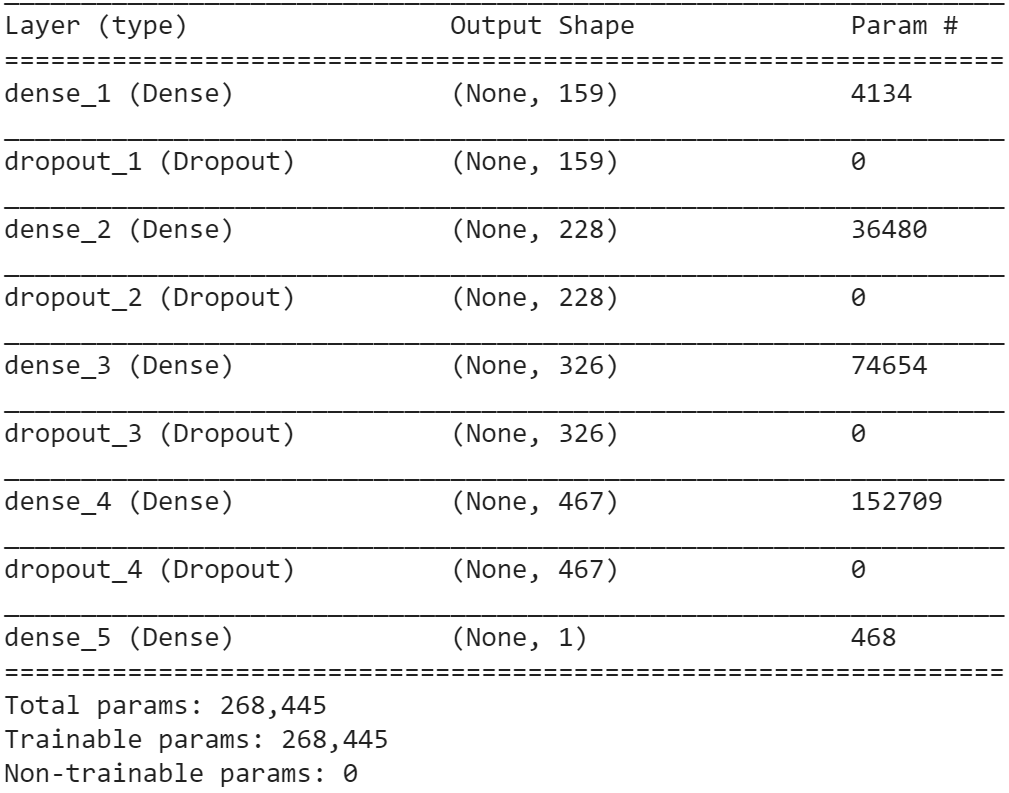
\includegraphics[width=0.47\textwidth]{figures/results/ann_summary.PNG}}
%     \caption{A summary of the MLP's structure.}
%     \label{fig:ann_summary}
%     \vspace{-10pt}
% \end{wrapfigure}
\InsertBoxR{3}{
    \parbox{0.5\linewidth}{
    \vspace{2mm}
    \fbox{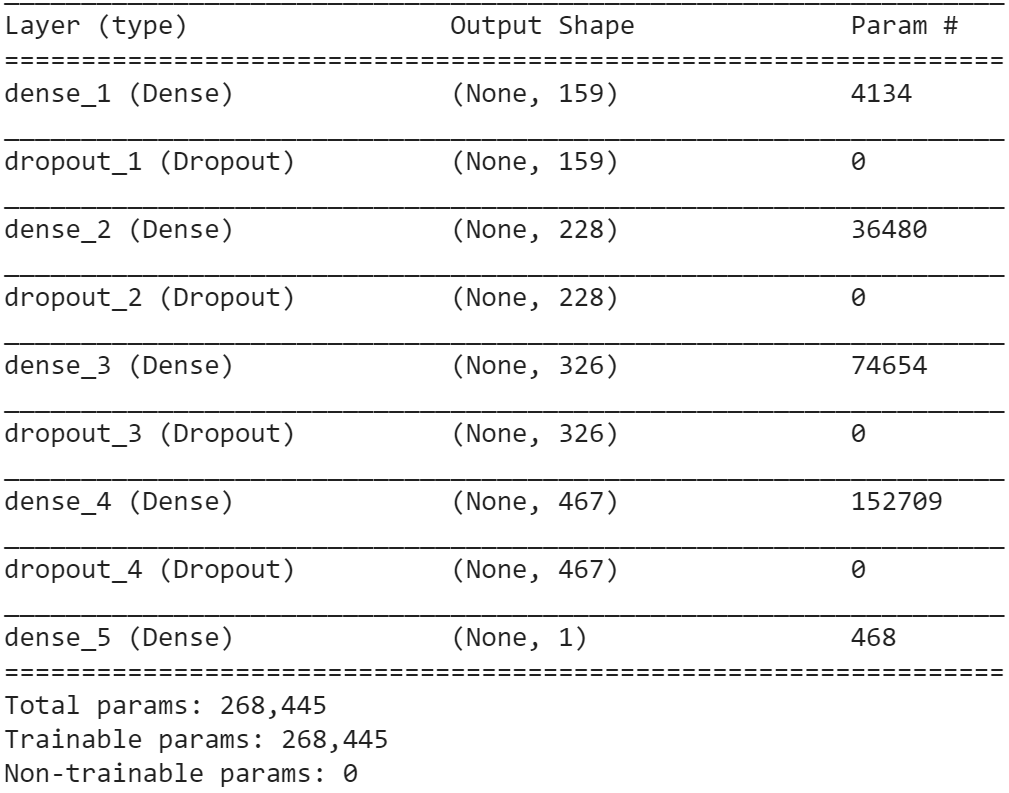
\includegraphics[width=0.47\textwidth]{figures/results/ann_summary.PNG}}
    \captionof{figure}{A summary of the MLP's structure.}
    \label{fig:ann_summary}}}[3]
A summary of the MLP model's structure is shown in Figure \ref{fig:ann_summary}.
The RMSE of the MLP model on the training, validation, and test sets were \annTrnRMSE{}, \annValRMSE{}, and \annTstRMSE{}, respectively.
Figure \ref{fig:ann_curve} shows the RMSE of the MLP model at each epoch on the training and validation sets.
This learning curve shows that most of the learning was done on the first iteration, and that the model had a difficult time learning useful information that will generalize well on the validation set after the first iteration.
The RMSE of the model exhibits a lot of oscillations, with the minimum validation error occurring at epoch 52.
Moreover, the MLP model was able to achieve an RMSSE of \annTstMonRMSSE{} for the 28-days ahead forecasts and was able to perform around 18.9\% better than the naive model.
Furthermore, the ME of the model on the test set was \annTstME{}, which means that the model has a tendency to under-forecast the target sale values.

The range of values that each hyperparameter of the model was optimized over, as well as their optimized values are shown in Table \ref{tab:ann_params}. 
The optimized MLP model contained four hidden fully-connected layers with 159, 228, 326, and 467 nodes, respectively.
Moreover, the optimized model did not include any batch normalization layers but had a dropout layer with a rate of \annParamsDropout{} after each fully-connected layer.
Additionally, for the training phase, the learning rate was optimized to be \annParamsLR{} with a decay rate of \annParamsDecay{} and the training batch size was optimized to be \annParamsBatch{}.


\section{LightGBM}
The LGBM model was able to achieve an RMSE of \lgbmTrnRMSE{}, \lgbmValRMSE{}, and \lgbmTstRMSE{} on the training, validation, and test sets, respectively.
The LGBM model was able to achieve the best performance on the test set compared to the other models.
From the learning curve of the model, shown in Figure \ref{fig:lgbm_curve}, it can be seen that the model's error plateaus around epoch 30, however, the model still continues to learn at a very low rate until epoch 122, where it reaches its best validation error, and then starts to overfit on the training set.
In addition, the ME and RMSSE of the 28-days ahead forecasts on the test set were \lgbmTstMonME{} and \lgbmTstMonRMSSE{}. respectively.
The RMSSE of the model shows that it was able to perform around 22.7\% better than the naive model.
Furthermore, the ME of the model shows that the model has a tendency to under-forecast the target sale values.

Table \ref{tab:lgbm_params} shows the range of values that each hyperparameter was optimized over and their optimized values.
The final LGBM model had a learning rate of \lgbmParamsLR{}, with \lgbmParamsFeatFrac{} fraction of features used to train each tree, and a lambda value of \lgbmParamsLambda{} for L2 regularization.
Moreover, the number of leaves for the model was chosen to be \lgbmParamsNleaves{} with a minimum data of \lgbmParamsMinData{} in each leaf.


\section{LSTM-LGBM Hybrid}
An LSTM model was chosen as the first component of the hybrid model in order to learn from the sales time-series data. 
Moreover, the best performing singular model between MLP and LGBM was used as the second component of the hybrid model.
Additionally, the optimal hyperparameters found previously for each singular model were used as the hyperparameters for each component.
The proposed hybrid model was able to obtain an RMSE of \hybTrnRMSE{} on the training set, \hybValRMSE{} on the validation set, and \hybTstRMSE{} on the test set for the 1-day ahead point forecasts.
These performances correspond to an RMSSE of \hybTrnRMSSE{}, \hybValRMSSE{}, and \hybTstRMSSE{} on the training, validation, and test sets, respectively.
Moreover, the RMSE and RMSSE of the hybrid model for the 28-days ahead forecasts on the test set were \hybTstMonRMSE{} and \hybTstMonRMSSE{}, respectively, which shows that the model was able to perform around 20.3\% better than the naive model.
Even though the hybrid model performed slightly worse than the singular LSTM model on the 1-day ahead forecasts, the hybrid model was able to obtain a slightly better performance on the 28-days ahead predictions, which shows that the second component, LGBM, was able to help counteract the effects of error propagation, which can be confirmed by comparing Figures \ref{subfig:lstm_sample28} and \ref{subfig:hyb_sample28}. 
On the other hand, the hybrid model was not able to beat the performance of the singular LGBM model.
Moreover, the ME of the model for the 28-days ahead forecasts on the test set was negative with a value of \hybTstMonME{}, which shows that the model is slightly under-forecasting the targets sale values.